\section{Evaluation}
We first presents the results from the live deployment of Argus.
We demonstrate the overhead of our tracing tool intruduced, regarding the storage, memory and CPU usage.
Then we list the softwares which trigger spinning wait cursors in MacOs and the root cause we figure out with our framework.
The list of real-world softwares includes TextEdit, CodEdit, Notes, Hopper Disassembler, Installer, Squel Pro, GetiPlayerAutomator.
At the end, we summaries the tedious work that our tool can take over from the user and make the diagnosis much easier in the wild.

\begin{figure}[tb]
    \centering
    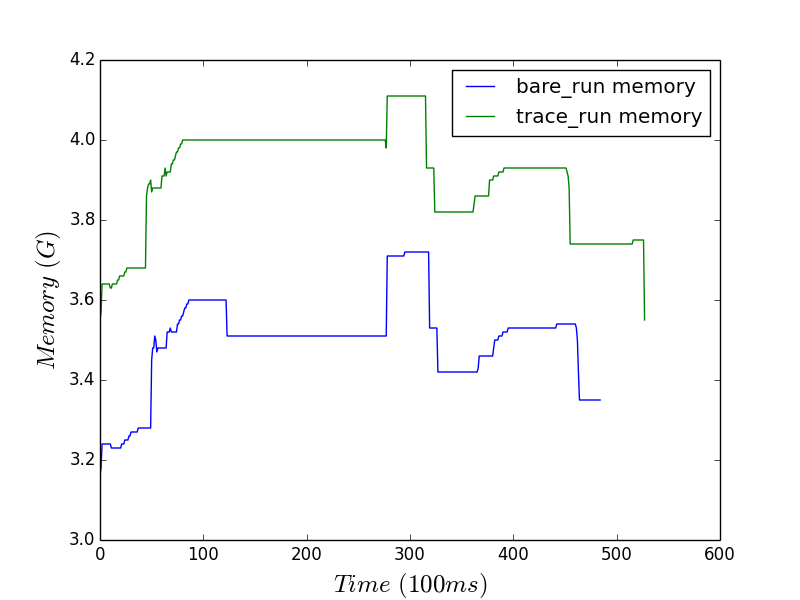
\includegraphics[width=1.0\linewidth]{ibench_memory_compare.png}
    \caption{Memory overhead with tracing.}
    \label{fig:ibench_memory_overhead}
\end{figure}

\begin{figure}[tb]
    \centering
    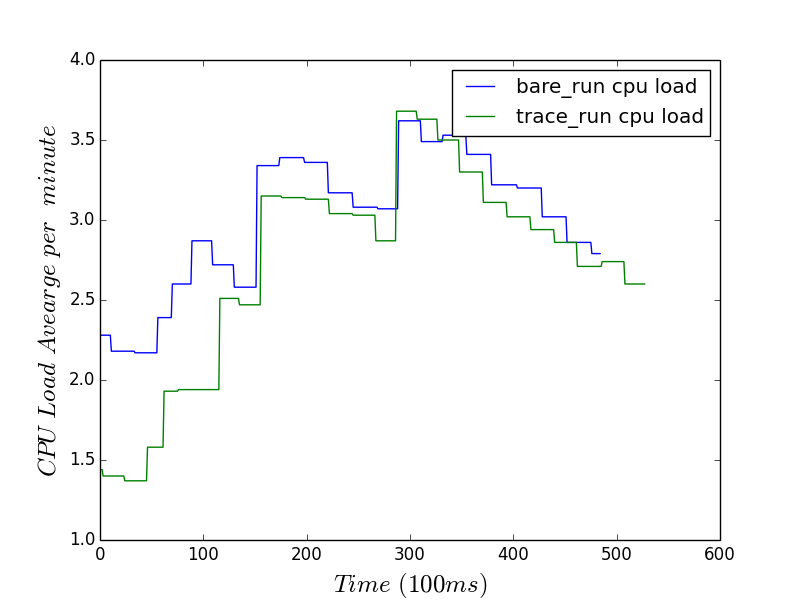
\includegraphics[width=1.0\linewidth]{ibench_cpuload_compare.png}
    \caption{CPU overhead with tracing.}
    \label{fig:ibench_cpu_overhead}
\end{figure}

\begin{itemize}
\item tracing overhead
	\begin{itemize}
	\item memory and CPU usage on top, while running ibench with and without our tracing enabled
	\item memory and CPU usage on top, while running the listed real world applications with and without our tracing enabled
	\item how much times it takes to filled the buffer we fixed 2G
	\item how many events recorded in the buffer
	\end{itemize}
\item number of edges and nodes in the graphs and portions of data the user need to examine to figure out the root cause.
\end{itemize}
